\subsubsubsubsection{Scheduling strategy}
\begin{figure}[h]
\centering
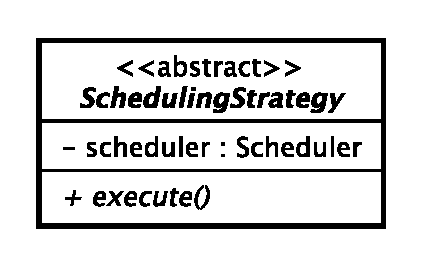
\includegraphics[scale=0.6,keepaspectratio]{images/solution/app/backend/scheduling_strategy.eps}
\caption{\pScheduling::SchedulingStrategy}
\label{fig:sd-app-scheduling-scheduling-strategy}
\end{figure}
\FloatBarrier
\begin{itemize}
  \item \textbf{\descr} \\
    An interface common to all supported scheduling algorithms. 
    A Scheduler objects use this interface to call the algorithm 
    is defined by a concrete class is derived by SchedulingStrategy.
  \item \textbf{\ops}
  \begin{itemize}
    \item[+] \texttt{\textit{execute()}} \\
Abstract method executes a scheduling algorithm.
  \end{itemize}
\end{itemize}
